\subsection{MatplotBench Example}
\subsubsection{Example 1}
\begin{minted}[fontsize=\footnotesize, linenos, frame=single]{markdown}
# Example 1 Inputs
## Task Instruction
**Task:**  
Utilize the following data columns from 'data.csv' to create a sunburst plot:\n- 'country': for the names of the countries,\n- 'continent': to indicate which continent each country is in,\n- 'lifeExp': showing the expected lifespan in each country,\n- 'pop': representing the population of each country.\nYour chart should:\n- Organize the data hierarchically, starting with continents and then breaking down into countries.\n- Use the population of each country to determine the size of its segment in the chart.\n- Color code each segment by the country's expected lifespan, transitioning from red to blue across the range of values.\n- Set the central value of the color scale to the average lifespan, weighted by the population of the countries.\n- Finally, include a legend to help interpret the lifespan values as indicated by the color coding.

---
## Environment
|--- data.csv 
\end{minted}


\begin{figure}[h!]
    \centering
    \begin{subfigure}[b]{0.45\linewidth}
        \centering
        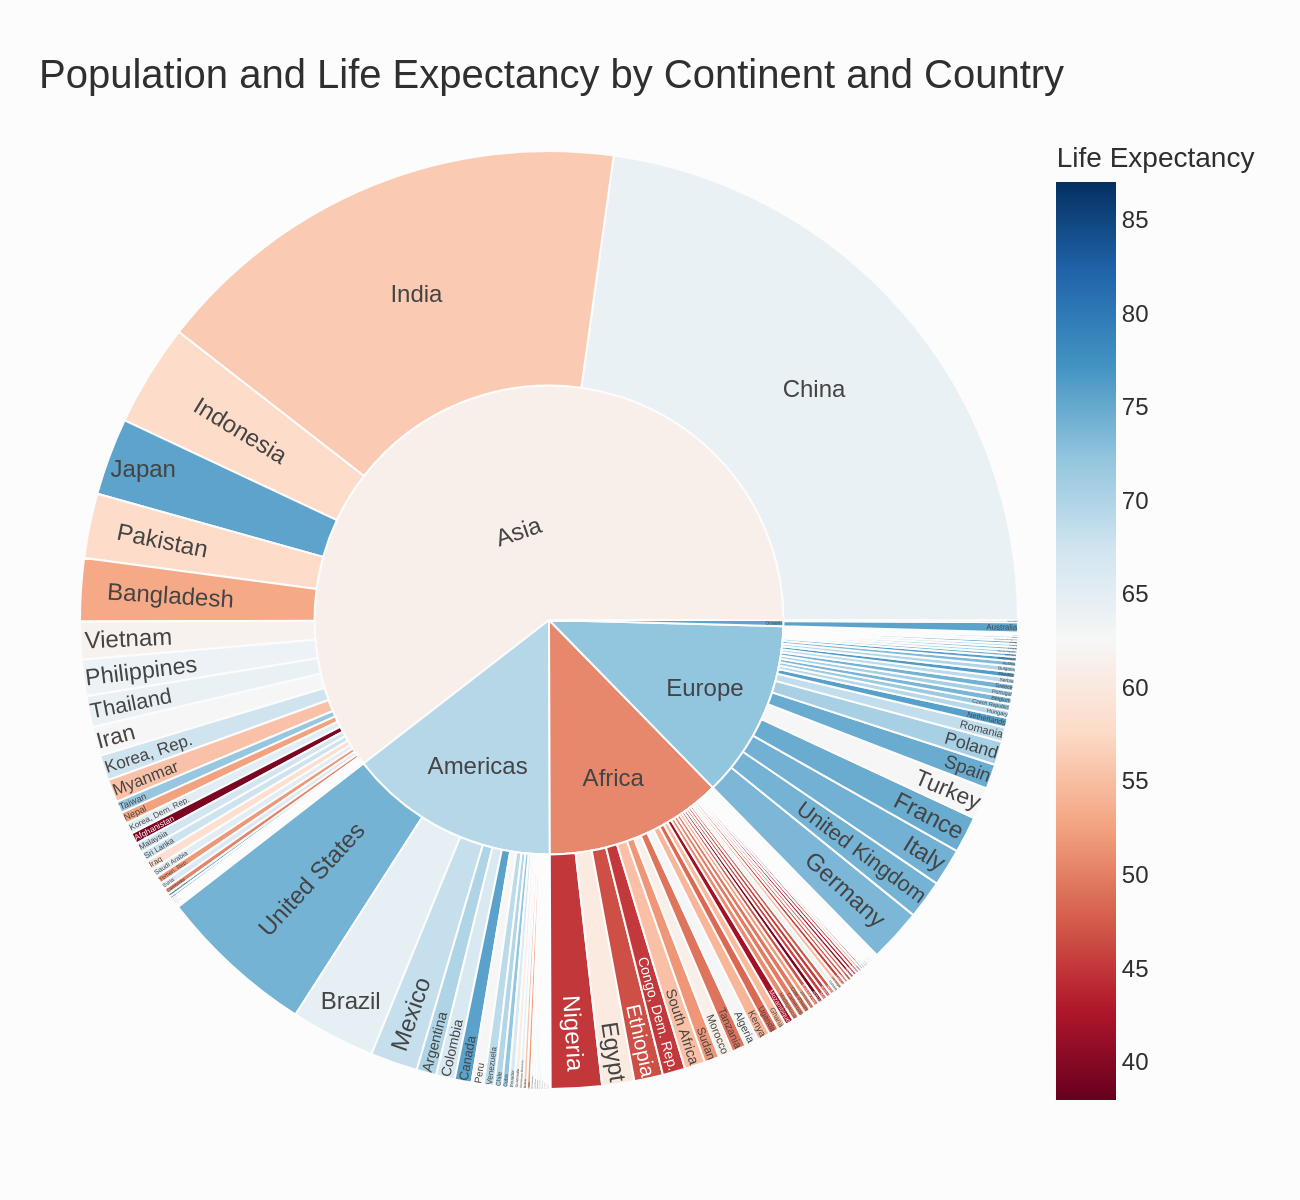
\includegraphics[width=\linewidth]{appendix/examples/95.png}
        \caption{\methodname{} Output}
    \end{subfigure}
    \hfill
    \begin{subfigure}[b]{0.51\linewidth}
        \centering
        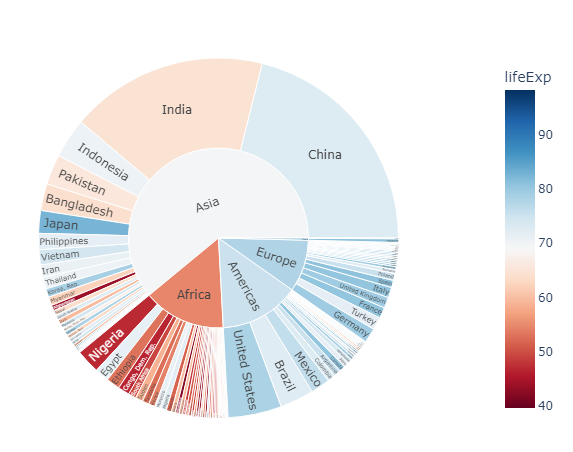
\includegraphics[width=\linewidth]{appendix/examples/gt-95.png}
        \caption{Ground Truth}
    \end{subfigure}
    \caption{Comparison between our generated sunburst plot and the reference output. 
    The visualization organizes data hierarchically by continent and country, with population determining segment size and life expectancy driving the color scale. 
    The results demonstrate full fidelity to the specification and highlight that our 
    system achieves a perfect score of \textbf{100/100}.}
    \label{fig:output-95-gt}
\end{figure}

\paragraph{Result Analysis.}
The sunburst visualization task required a multi-level hierarchical organization of the data, 
starting from continents and further breaking down into individual countries. Our method 
successfully utilized population size to determine segment area and applied a red-to-blue 
color scale based on life expectancy (Figure~\ref{fig:output-95-gt}), with the weighted average lifespan as the central pivot 
for normalization. This design ensured both interpretability and faithful representation of 
the dataset’s structure. The resulting chart aligns precisely with the ground truth and 
provides an intuitive overview of demographic and geographic patterns, achieving a perfect 
score of \textbf{100/100}.
